\documentclass{beamer}
\usetheme{Marburg}
\usepackage{tikz}
\usepackage{color,soul}
\usepackage{tabularx}
\def\Put(#1,#2)#3{\leavevmode\makebox(0,0){\put(#1,#2){#3}}}
\newcommand{\fmax}{f_\mathrm{max}}
\newcommand{\bx}{\mathbf{x}}
\newcommand{\by}{\mathbf{y}}
\newcommand{\bA}{\mathbf{A}}
\newcommand{\bI}{\mathbf{I}}
\newcommand{\bSig}{\mathbf{\Sigma}}
\newcommand{\rT}{\mathrm{T}}
\newcommand{\abs}[1]{\left\lvert #1\right\rvert}
\newcommand{\norm}[1]{\left\lvert\left\lvert #1\right\rvert\right\rvert}
\title{06 22313 Computational Tools for Modelling and Analysis}
\subtitle{Introductory Lecture}
\author{Dr Iain Styles (I.B.Styles@bham.ac.uk)}
\institute{School of Computer Science, University of Birmingham}
\date{October 12 2015}

\begin{document}

\begin{frame}
  \titlepage
\end{frame}

\begin{frame}{Outline}
  \tableofcontents
\end{frame}

%%%%%%%%%%%%%%%%%%%%%%%%%%%%%%%%%%%%%%%%%%%%%%%%%%%%%%
\section{Introduction}
\subsection{What are the aims?}

\begin{frame}{Course Aims}
  \begin{itemize}
    \item Introduce concepts, techniques and tools for the computational modelling and analysis of data from medicine and biology.
    \item Survey methods for statistical data analysis, machine learning, optimisation, classification, cluster analysis, data reduction and image analysis.
    \item Provide both theoretical background and practical experience of implementing and applying the techniques.
  \end{itemize}
\end{frame}

\subsection{Administrative Matters}
\begin{frame}{Who's teaching the course?}
  \begin{minipage}{0.32\textwidth}
    \begin{center}
      Iain Styles\\ 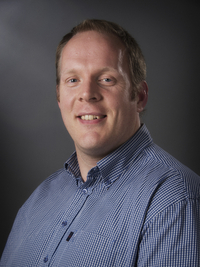
\includegraphics[width=0.9\textwidth]{is}\\I.B.Styles\dots
    \end{center}
  \end{minipage}
  \begin{minipage}{0.32\textwidth}
    \begin{center}
      Hamid Dehghani\\ 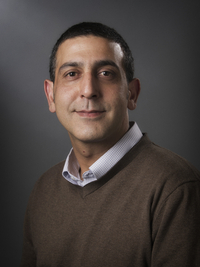
\includegraphics[width=0.9\textwidth]{hd}\\H.Dehghani\dots
    \end{center}
  \end{minipage}
  \begin{minipage}{0.32\textwidth}
    \begin{center}
      Ela Claridge\\ 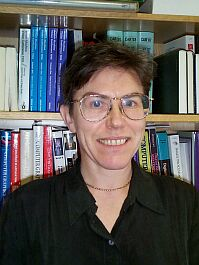
\includegraphics[width=0.9\textwidth]{ec}\\E.Claridge\dots
    \end{center}
  \end{minipage}
  \begin{center}
    \dots @cs.bham.ac.uk
  \end{center}
\end{frame}

\begin{frame}{Assessment}
  Continuous Assessment (30\%)
  \begin{itemize}
    \item Nine weekly assessments: use the ``technique of the week'' to study a biomedical dataset, write a 2-page report on your findings.
  \end{itemize}

  Examination (70\%)
  \begin{itemize}
    \item 90 minute exam in May 2016.
    \item Pass mark is 50\%
  \end{itemize}
\end{frame}

\subsection{What will we cover?}
\begin{frame}{}
  So what we will we cover?
\end{frame}

\begin{frame}{Mathematical Essentials: Linear Algebra and Basic Frequentist Statistics}
  \begin{minipage}[t]{0.45\textwidth}
    \begin{center}
      Linear Equations
      \begin{eqnarray*}
        3x+2y&=&7 \\
        x-4y&=& 4
      \end{eqnarray*}
      \begin{itemize}
      \item Representation as matrices
      \item Methods of solution
      \item Working with MATLAB
      \end{itemize}
    \end{center}
  \end{minipage}
  \begin{minipage}[t]{0.45\textwidth}
    \begin{center}
      Random Variables
      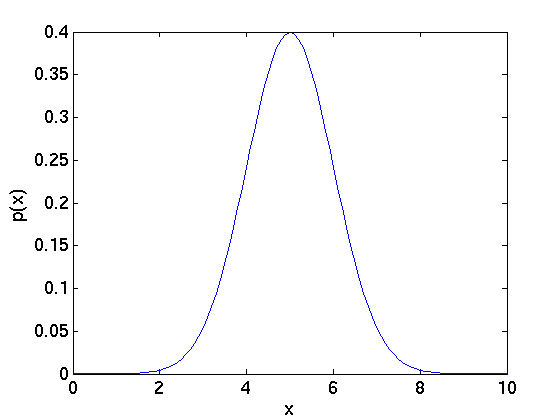
\includegraphics[width=\textwidth]{gaussian}
      \begin{itemize}
        \item Basic definitions
        \item Distributions
        \item Working with MATLAB
      \end{itemize}
    \end{center}
  \end{minipage}
\end{frame}

\begin{frame}{Fitting Models to Data}
  Rate of unimolar (first-order) chemical reactions
  \begin{eqnarray*}
    \mbox{H}_2 \mbox{O}_2  & \rightarrow & \; \mbox{H}_2\mbox{O}  + \frac{1}{2}\mbox{O}_2 \\
    \log [\mbox{H}_2 \mbox{O}_2] &=& = -kt+\log [\mbox{H}_2 \mbox{O}_2]_0
  \end{eqnarray*}
  \begin{center}
    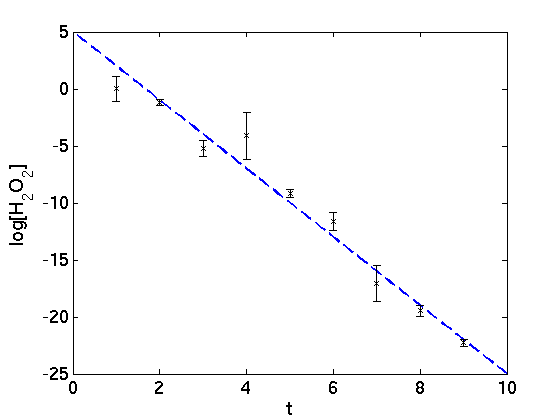
\includegraphics[width=0.5\textwidth]{reaction}
  \end{center}
\end{frame}

\begin{frame}{Image Reconstruction and Inverse Problems}
  \begin{minipage}[t]{0.45\textwidth}
    \begin{center}
      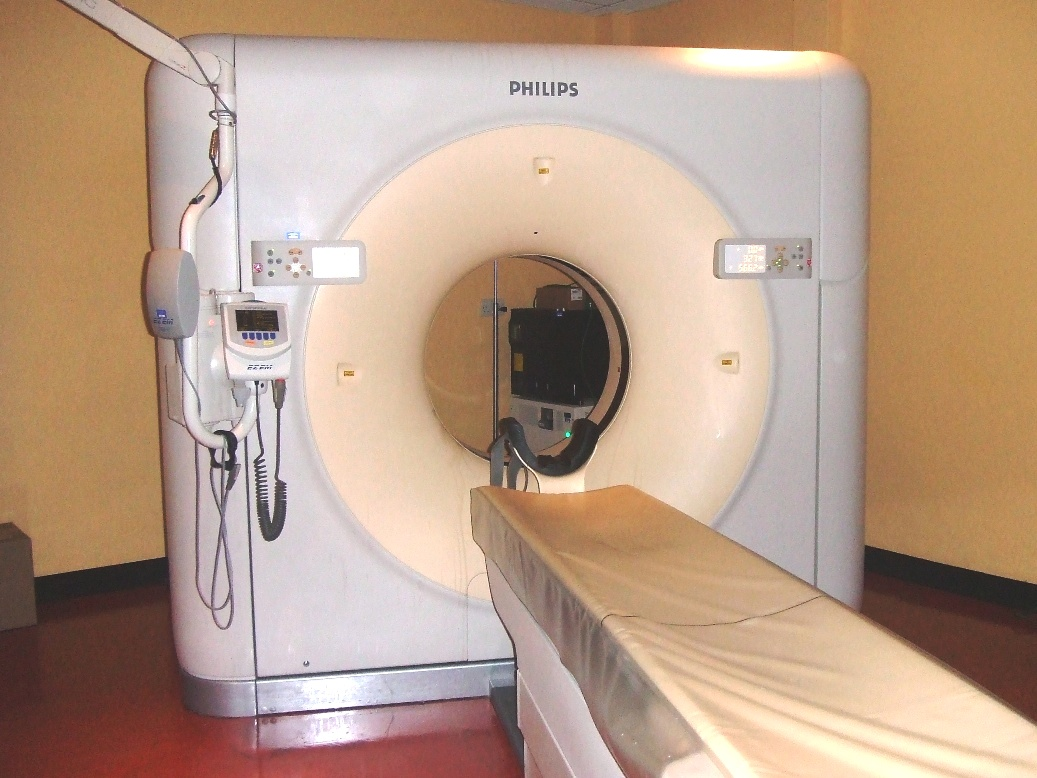
\includegraphics[width=0.9\textwidth]{ctscanner}\\
    \end{center}
  \end{minipage}
  \begin{minipage}[t]{0.45\textwidth}
    \begin{center}
      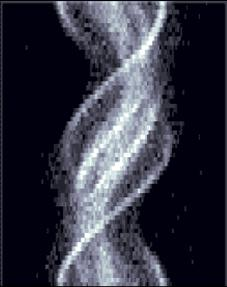
\includegraphics[angle=90,width=0.9\textwidth]{sinogram}
    \end{center}
  \end{minipage}
  \begin{center}
    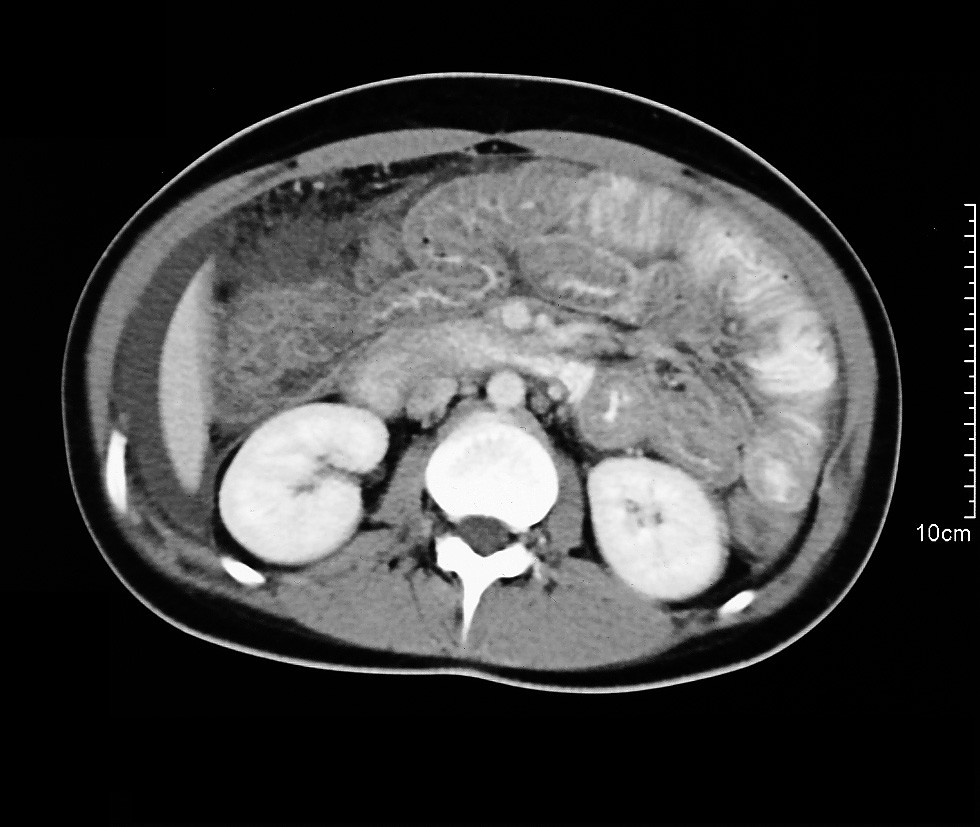
\includegraphics[width=0.5\textwidth]{ctimage}
  \end{center}
\end{frame}

\begin{frame}{Dimensionality Reduction}
  
\includegraphics[width=0.55\textwidth]{pcaex1}\\
  \hspace{0.45\textwidth}
\includegraphics[width=0.55\textwidth]{pcaex2}
\end{frame}

\begin{frame}{Classification}
  \begin{center}
    
\includegraphics{classification}\\
  \end{center}
\end{frame}

\begin{frame}{Clustering}
    \begin{center}
      
\includegraphics[width=\textwidth]{simpleclusters}\\
      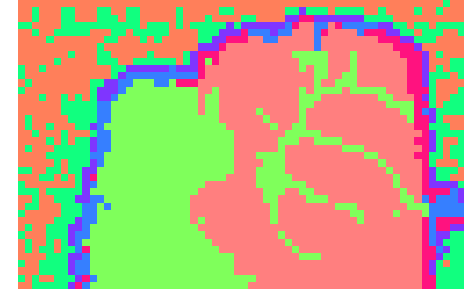
\includegraphics[width=0.6\textwidth]{cluster}
    \end{center}
\end{frame}

\begin{frame}{Image Segmentation}
    \begin{center}
      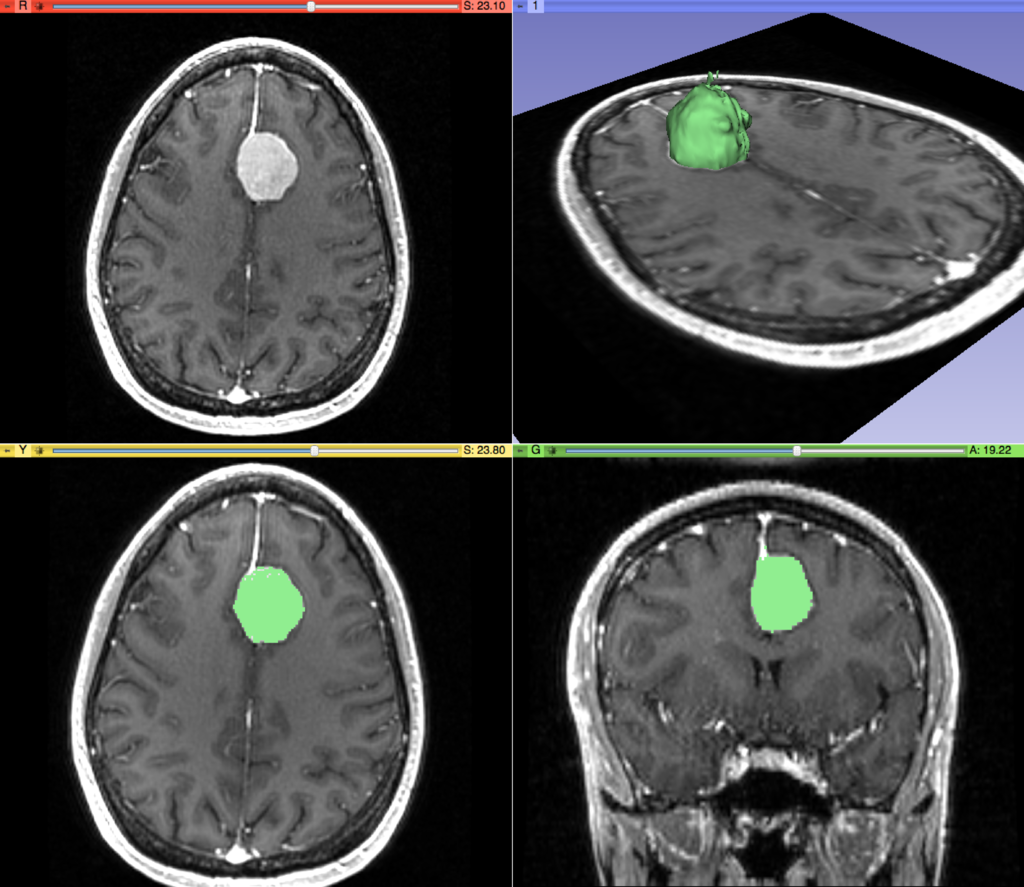
\includegraphics[width=0.9\textwidth]{mrisegmentation}
    \end{center}
\end{frame}

\begin{frame}{Image Registration}
    \begin{center}
      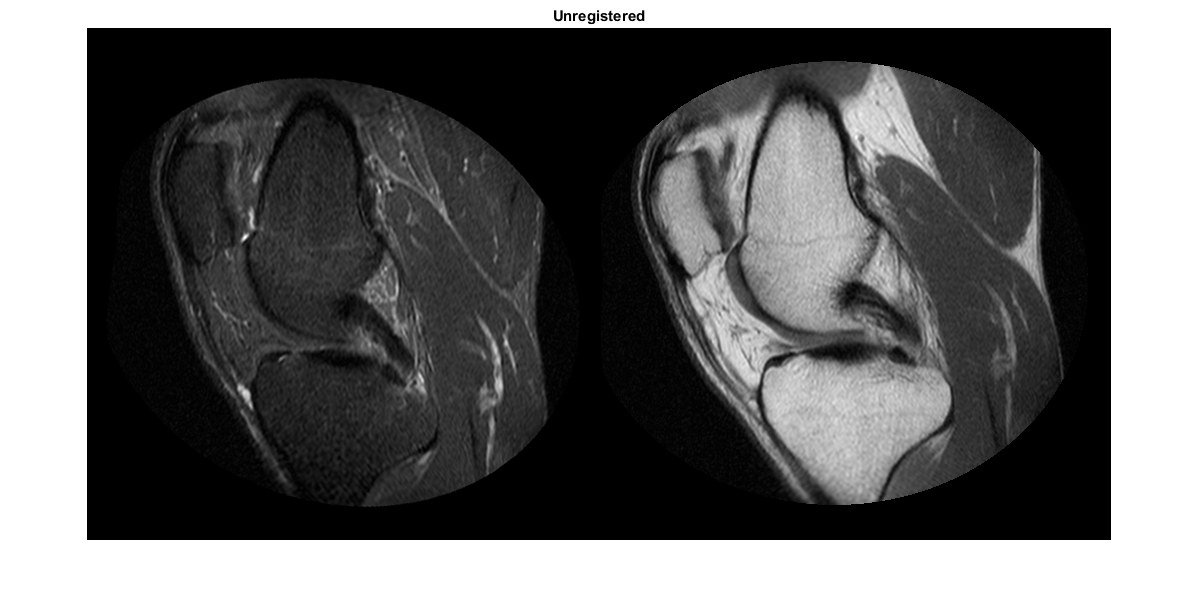
\includegraphics[width=\textwidth]{registration1}\\
      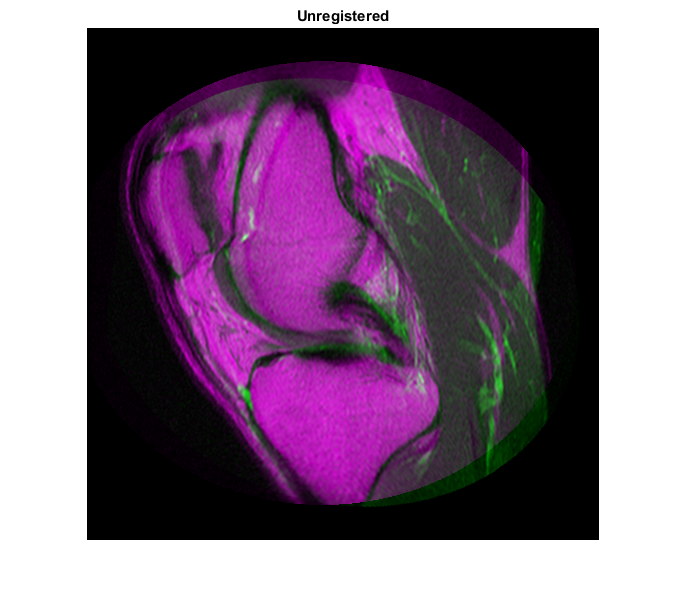
\includegraphics[width=0.5\textwidth]{registration2}
      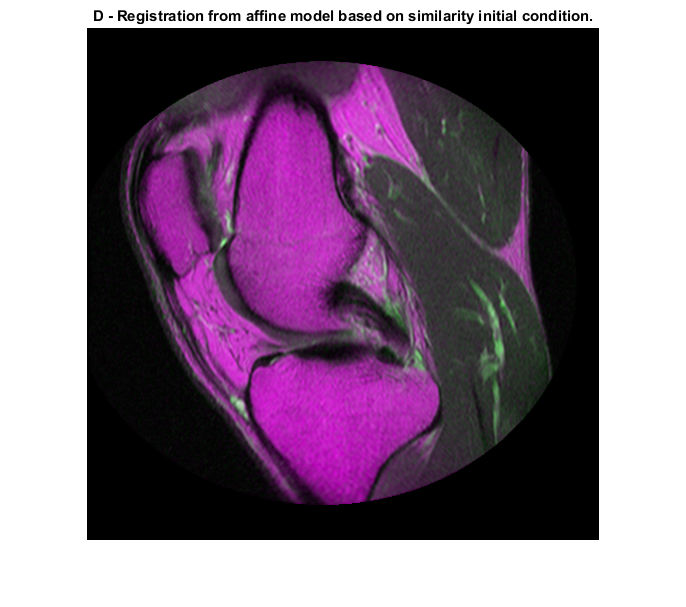
\includegraphics[width=0.5\textwidth]{registration3}
    \end{center}
\end{frame}

\begin{frame}{Tracking and Motion}
  \begin{center}
    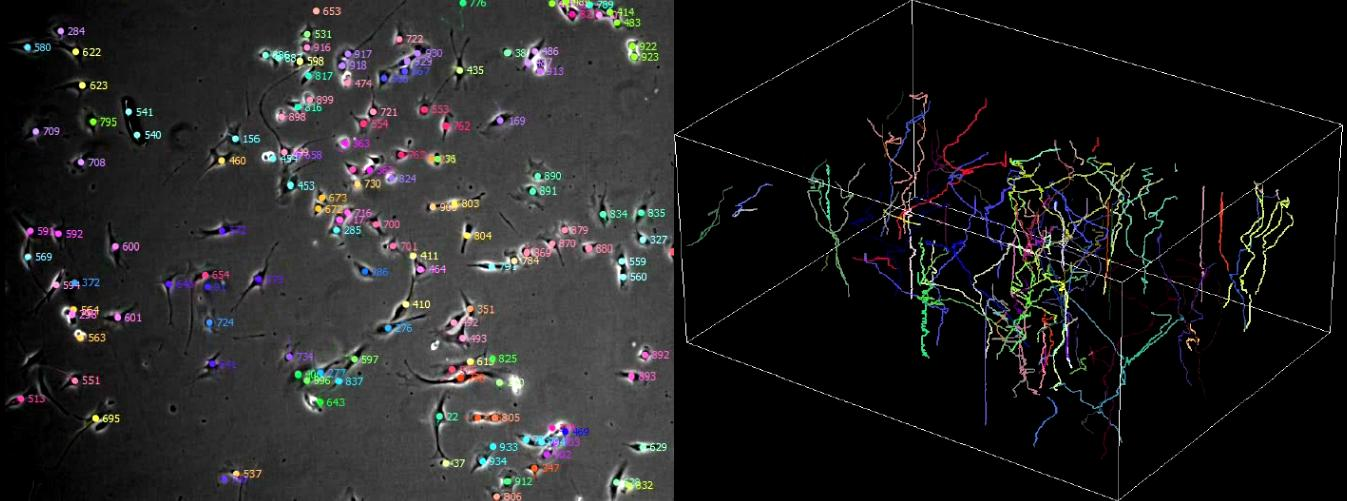
\includegraphics[width=\textwidth]{tracking}
  \end{center}
\end{frame}

%%%%%%%%%%%%%%%%%%%%%%%%%%%%%%%%%%%%%%%%%%%%%%%%%%%%%%
\section{Mathematics and Matlab}

\begin{frame}
\end{frame}

\begin{frame}{Motivation}
    \begin{itemize}
      \item Quantitative analysis of quantitative data requires mathematics
      \item The core basic concepts are:
        \begin{itemize}
          \item Simultaneous linear equations
          \item Random variables
        \end{itemize}
      \item We also need to know how to use tools for working with data and mathematics
      \item We will be using MATLAB: MATrix LABoratory software for this.
        \begin{itemize}
          \item MATLAB is a ``domain-specific'' programming language with a ``friendly'' interactive interface.
          \item We will learn how to ``do maths'' in MATLAB and develop some basic computer programming skills.
        \end{itemize}
    \end{itemize}
\end{frame}

\subsection{Linear Equations}
\begin{frame}{Simultaneous Linear Equations}
  \begin{itemize}
    \item Consider the following set of simultaneous linear equations:
      \begin{eqnarray}
        2x-y &=& 3 \label{sima}\\
        x+y &=&3 \label{simb}
      \end{eqnarray}
    \item The solution to these is easy to guess but can be done systematically.
    \item Add eq.\eqref{sima} to eq.\eqref{simb}:
      \begin{eqnarray*}
        (2x-y)+(x+y) &=& 3+3 \\
        3x&=&6\\
        x&=&2
      \end{eqnarray*}
      \item and by substitution $y=1$.
        \end{itemize}
\end{frame}


\begin{frame}{Solving Linear Equations}
  \begin{itemize}
    \item Manual solution is fine for small problems, but hugely impractical for even moderately large systems, e.g. 10,000 equations with as many unknowns.
    \item \textbf{Linear algebra}: rules and techniques for solving linear equations efficiently and compactly.
    \item Represent linear equations in terms of
      \begin{itemize}
        \item Vectors: which represent some ``object'', say $\bx$ and $\by$
        \item Matrices: which represent some ``transformation'', say $\bA$
      \end{itemize}
    \item Example: simple photographic imaging 
  \end{itemize}
\end{frame}

\begin{frame}{Linear Equations $\leftrightarrow$ Matrices and Vectors}
  \begin{eqnarray*}
    2x-y &=& 3 \label{sima}\\
    x+y &=&3 \label{simb}
  \end{eqnarray*}
  In object-transformation paradigm we have vectors
  \begin{equation*}
      \bx = \begin{pmatrix}x\\y\end{pmatrix}\quad\mbox{and}\quad \by = \begin{pmatrix}3\\3\end{pmatrix}
  \end{equation*}
  The linear equations are then represented as
  \begin{equation*}
    \by=\bA\bx\quad\mbox{where}\quad \bA=\begin{pmatrix}2 & -1\\1 &1\end{pmatrix}
  \end{equation*}
  is the ``transformation''.
\end{frame}

\begin{frame}{Reversing Transformations}
  \begin{itemize}
    \item Solving a set of linear equations $\equiv$ reversing the transformation.
    \item If a transformation is reversible there there exists another transformation matrix $\bA^{-1}$ that ``inverts'' it such that:
      \begin{equation*}
        \bA^{-1}\bA\bx = \bx \quad \mbox{or}\quad\bA^{-1}\bA=\bI= \begin{pmatrix}1 & 0 \\0 & 1\end{pmatrix}
      \end{equation*}
      \item We will not dwell on how to find $\bA^{-1}$ but note that for our example
        \begin{equation*}
          \begin{pmatrix}\frac{1}{3}&\frac{1}{3}\\-\frac{1}{3}&\frac{2}{3}\end{pmatrix}\begin{pmatrix}2 & -1\\1 &1\end{pmatrix}=\begin{pmatrix}1 & 0\\0 &1\end{pmatrix}
        \end{equation*}
      \item How do we do this in the Computer?
  \end{itemize}
\end{frame}

\begin{frame}{Irreversible Transformations}
  Inverse can only be found exactly/uniquely if:
  \begin{itemize}  
  \item The number of unknowns is equal to the number of equations.
    \begin{itemize}
    \item More unknowns than equations $\rightarrow$ non-unique solution (underdetermined)
    \item More equations than unknowns $\rightarrow$ non-exact solution (overdetermined)
    \end{itemize}
  \item The equations (row of $\bA$) are linearly independent.
  \item Examples:
  \end{itemize}
  \begin{minipage}[t]{0.45\textwidth}
    \begin{eqnarray*}
      2x-y+z & = & 3 \\
      x+y-z & = & 3 
    \end{eqnarray*}
  \end{minipage}
  \begin{minipage}[t]{0.45\textwidth}
    \begin{eqnarray*}
      2x-y &=& 3\\
      x+y & = & 3 \\
      x-y & = & 0
    \end{eqnarray*}
  \end{minipage}

  How does the computer deal with these cases?
\end{frame}







\subsection{Random Variables}
\begin{frame}{Random Variables}
  \begin{itemize}
    \item A random variable is one that is subject to some degree of nondeterminism
      \begin{itemize}
        \item Bus/train times
        \item Physical measurements and quantities derived from them
      \end{itemize}
    \item Characterised by a \textbf{probability density function}
      \begin{itemize}
        \item Describes the ``distribution'' of values that the variable can take
        \item Examples: Gaussian (normal); Poisson; Log normal.
      \end{itemize}
  \end{itemize}
\end{frame}

\begin{frame}{Probability Density Function}
  \begin{center}
    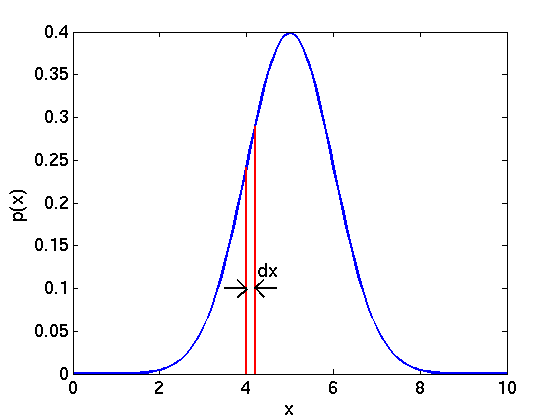
\includegraphics[width=0.7\textwidth]{distribution}
  \end{center}
  $\int_{x_1}^{x_2}p(x)\mathrm{d}x$ (area under curve) is probability that $x$ is in interval $[x_1,x_2]$ [total area is 1].
\end{frame}

\begin{frame}{Characterics of PDFs}
  Given a collection of $N$ numerical values ${x_1, x_2,\dots, x_N}$ drawn from a distribution it is common to compute:
  \begin{itemize}
    \item Arithmetic mean: $\bar x = \frac{1}{N}\sum_{i=1}^N x_i$
    \item Median: sort the values in order from lowest to highest, median is the ``middle'' value, or the mean of the middle pair if $N$ is even.
    \item Mode: the most commonly occurring value.
    \item Variance: $\mbox{var}(x)=\sum_{i=1}^N \left(\bar x -x_i\right)^2$
    \item Standard deviation: $\sigma(x)=\sqrt{\mbox{var}(x)}$
    \item But take care about the particular form of your distribution $\dots$
  \end{itemize}
\end{frame}

\begin{frame}{The Normal Distributions}
  \begin{center}
    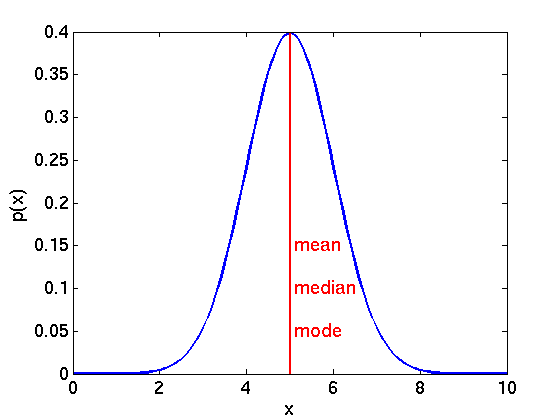
\includegraphics[width=0.7\textwidth]{normalaverages}
    \begin{eqnarray*}
      p(x) &=& \frac{1}{\sigma\sqrt{2\pi}}\ e^{-\frac{\left(x-\mu\right)^2}{2\sigma^2}}\\
      \mbox{Mean}&:& \mu\\
      \mbox{Median}&:& \mu\\
      \mbox{Mode}&:& \mu
    \end{eqnarray*}
  \end{center}
\end{frame}

\begin{frame}{The Lognormal Distribution}
  \begin{center}
    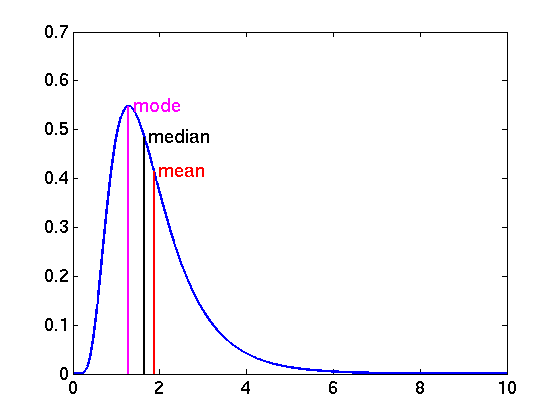
\includegraphics[width=0.7\textwidth]{lognormalaverages}
    \begin{eqnarray*}
      p(x) &=& \frac{1}{x\sigma\sqrt{2\pi}}\ e^{-\frac{\left(\ln x-\mu\right)^2}{2\sigma^2}}\\
      \mbox{Mean}&:& e^{\mu+\sigma^2/2}\\
      \mbox{Median}&:& e^\mu\\
      \mbox{Mode}&:& e^{\mu-\sigma^2}
    \end{eqnarray*}
  \end{center}
\end{frame}

\end{document}

